\chapter{تناظر التبادل، واللف المغزلي، وعلامتا السالب}

\section{ملء الأغلفة ومسألة اللف المغزلي--الإحصاء}

تبدأ مراجعة نموذج الأغلفة بخاصيتين مرتبطتين بالإلكترونات. فللإلكترون لف مغزلي مقداره نصف، وله إسقاطان مغزليان عديمَا الأبعاد
\begin{equation}
m_s=+\frac12,
\qquad
m_s=-\frac12,
\end{equation}
وتخضع الإلكترونات لمبدأ استبعاد باولي. هاتان الحقيقتان مرتبطتان، لكنهما ليستا العبارة نفسها.

عبارة ``الحالة نفسها'' تحتاج إلى تدقيق. لا يجوز لإلكترونين أن يشغلا الحالة الأحادية الجسيم الكاملة نفسها. ومع ذلك، يجوز لإلكترونين أن يشتركا في مدار مكاني واحد عندما تختلف حالتا لفهما المغزلي. في تقريب الإلكترونات المستقلة لذرة الهيليوم، يشغل كلا الإلكترونين أدنى مدار مكاني، أحدهما بلف مغزلي إلى أعلى والآخر بلف مغزلي إلى أسفل. وعلى نحو أدق، فإن البديلين ``الأول إلى أعلى والثاني إلى أسفل'' و``الأول إلى أسفل والثاني إلى أعلى'' ينتميان إلى حالة لف مغزلي متشابكة لإلكترونين.

هذا ليس إلا تقريب نموذج الأغلفة القديم. فهو يهمل التآثر بين الإلكترونات ويُستخدم هنا لبساطة العد. في الليثيوم، يملأ الإلكترونان الأولان أدنى مدار مكاني بلفين مغزليين متعاكسين. أما الثالث فلا يمكنه دخول أيٍّ من هاتين الحالتين الكاملتين، ولذا يجب أن يشغل مدارًا أعلى.

الخطوة التالية هي مخطط العزم الزاوي المداري المألوف. وتسمى القطاعات ذات
\begin{equation}
\ell=0,\qquad \ell=1,\qquad \ell=2
\end{equation}
حالات \(S\) و\(P\) و\(D\). ولقيمة ثابتة من \(\ell\) يوجد
\begin{equation}
2\ell+1
\end{equation}
من الحالات المدارية، ولذلك
\begin{equation}
\ell=0\Rightarrow 1,
\qquad
\ell=1\Rightarrow 3,
\qquad
\ell=2\Rightarrow 5.
\end{equation}
وتوجد في مسألة كولوم انحلالات إضافية: إذ يمكن للمستويات الشعاعية من قطاعات \(\ell\) مختلفة أن تكون لها الطاقة نفسها. وفي حجة ملء الأغلفة، يحتوي الغلاف التالي على مدار واحد من نوع \(S\) وثلاثة مدارات من نوع \(P\). ولذلك فإن لديه
\begin{equation}
1+3=4
\end{equation}
من الحالات المكانية. ويضاعف اللف المغزلي هذا العدد:
\begin{equation}
2(1+3)=8.
\end{equation}

تُملأ هذه الحالات الثماني الكاملة للإلكترون الواحد في التدرج البسيط من الليثيوم حتى النيون. وبعد الغلاف المغلق، يكون للصوديوم من جديد إلكترون خارجي واحد، ولهذا تجعله هذه الصورة التقريبية يشبه الليثيوم. ليست الكيمياء هي المقصود. فالمغزى أن اللف المغزلي نصف الصحيح والاستبعاد يظهران معًا.

وتوفر الفوتونات المقابلة. فلها لف مغزلي صحيح ولا تخضع لقاعدة استبعاد. وتقابل الموجة الكهرومغناطيسية الكلاسيكية عددًا كبيرًا من الفوتونات يشغل النمط نفسه. يمكن للبوزونات أن تتراكم في حالة مشتركة، في حين لا تستطيع الفرميونات المتماثلة أن تشغل حالة كاملة واحدة أكثر من مرة. والسؤال هو ما إذا كان من الممكن أن يكون هذان الاقترانان على غير ذلك: لف مغزلي نصف صحيح من دون استبعاد، أو لف مغزلي صحيح مع استبعاد. في ثلاثة أبعاد مكانية، تقول علاقة اللف المغزلي--الإحصاء: لا. وتحتاج العبارة المألوفة إلى تقييد في بعد مكاني واحد وبعدين مكانيين، ولا تُبذل هنا أي محاولة لإثبات النتيجة في نظرية الحقول.

\begin{classroomqa}
\lecturetimestamp{00:11:48}
\audiencequestion{هل يوجد حد أقصى لعدد الكمات البوزونية التي يمكن أن تشغل حالة واحدة؟}
\lecturerresponse{لا. ليس للبوزونات حد للإشغال، وهي تميل إلى التراكم في الحالة نفسها.}
\end{classroomqa}

\section{دوال الموجة متعددة الجسيمات}

سيُتناول هذا الارتباط عبر علامتي سالب، إحداهما من التبادل والأخرى من الدوران. لنبدأ بالتبادل، ولنُهمل اللف المغزلي مؤقتًا.

لتدل \(x_i\) على موضع الجسيم \(i\). فالرمز السفلي وسم للجسيم، لا مركبة ديكارتية؛ وقد اختُزلت الإحداثيات المكانية الثلاثة في الرمز المفرد \(x_i\). وأساس الموضع لعدد \(n\) من الجسيمات هو
\begin{equation}
\lvert x_1,x_2,\ldots,x_n\rangle.
\end{equation}
وبالنسبة إلى الحالة المجردة \(\lvert\Psi\rangle\)، تكون دالة الموجة الإحداثية
\begin{equation}
\psi(x_1,x_2,\ldots,x_n)
=
\langle x_1,x_2,\ldots,x_n\mid\Psi\rangle.
\end{equation}
ومربع مقدارها،
\begin{equation}
\bigl\lvert\psi(x_1,x_2,\ldots,x_n)\bigr\rvert^2,
\end{equation}
هو كثافة الاحتمال المشتركة لإيجاد الجسيم \(1\) عند \(x_1\)، والجسيم \(2\) عند \(x_2\)، وهكذا.

والآن افترض أن الجسيمات متماثلة. تخيل أولًا أن أحد الإلكترونين مطلي بالأزرق والآخر بالأحمر. عندئذ يمكن تمييز ``أزرق عند \(x_1\)، وأحمر عند \(x_2\)'' عن ``أزرق عند \(x_2\)، وأحمر عند \(x_1\).'' لكن الإلكترونات الفعلية لا تحمل ألوانًا كهذه ولا وسومًا فردية. إن تبديل التسميات الاصطلاحية لا يمكن أن يخلق ترتيبًا فيزيائيًا جديدًا.

لا يغير الطور الكلي الاحتمالات ولا القيم المتوقعة. ولذلك، بالنسبة إلى حالة تقع في قطاع تبادل محدد، يجوز لدالة الموجة الإحداثية أن تحقق
\begin{equation}
\psi(x_2,x_1)=\eta\,\psi(x_1,x_2),
\qquad
\lvert\eta\rvert=1.
\end{equation}
ويعيد تطبيق التبادل نفسه مرتين الوسائط الأصلية ويعطي
\begin{equation}
\eta^2=1,
\end{equation}
ومن ثم فإن القيم الذاتية الممكنة للتبادل هي
\begin{equation}
\eta=+1
\qquad\hbox{or}\qquad
\eta=-1.
\end{equation}

\editorialnote{لا يحدد جبر التبادل المزدوج القيم الذاتية الممكنة إلا بعد افتراض أن للحالة سلوك تبادل محددًا. أما القيد الإضافي القائل إن الحالات المسموح بها لنوع معيّن تقع في قطاع تبادل واحد فهو قاعدة فيزيائية؛ ولا يترتب على \(\eta^2=1\) وحده. وينطبق التقييد نفسه على حجة الاستبعاد أدناه: فمضادة التناظر تستلزم الاستبعاد بعد اختيار القطاع الفرميوني، لكن جبر التبادل بذاته لا يختار ذلك القطاع.}

بالنسبة إلى البوزونات، تكون دوال الموجة المسموح بها متناظرة،
\begin{equation}
\psi_B(x_1,x_2)=\psi_B(x_2,x_1),
\end{equation}
في حين أنها بالنسبة إلى الفرميونات مضادة للتناظر،
\begin{equation}
\psi_F(x_1,x_2)=-\psi_F(x_2,x_1).
\end{equation}
وتكون إشارة السالب غير مرئية عندما تضرب الحالة كلها، لكنها تهم حين تُجمع السعات. وهكذا يكتسب تناظر التبادل نتائج قابلة للرصد.

\section{الجداءات، والمجاميع، والاستبعاد}

انظر أولًا إلى جسيمين مسندين إلى المدار الأحادي الجسيم نفسه \(\psi_0\). فيكون جداؤهما
\begin{equation}
\psi_0(x_1)\psi_0(x_2).
\end{equation}
ويعطي تبديل إحداثيي الجسيمين
\begin{equation}
\psi_0(x_2)\psi_0(x_1)
=
\psi_0(x_1)\psi_0(x_2).
\end{equation}
وقيم دالة الموجة أعداد لا مؤثرات، لذا فإن العوامل تتبادل. وجدء الحالة نفسها متناظر. وهو صيغة بوزونية مسموح بها، لكنه لا يستطيع وصف فرميونين متماثلين.

بعد ذلك، أسند الجسيمين إلى مدارين أحاديي الجسيم مختلفين:
\begin{equation}
\psi_0(x_1)\psi_1(x_2).
\end{equation}
فينتج عن التبادل
\begin{equation}
\psi_0(x_2)\psi_1(x_1).
\end{equation}
وبالنسبة إلى دالتين متميزتين، فإن الجداء بعد التبادل ليس، بوجه عام، التعبير الأصلي ولا سالبه. لذلك لا يملك الجداء المحض أيًا من تناظري التبادل المطلوبين. وهذا لا يمنع أن يشغل أحد الجسيمين \(\psi_0\) بينما يشغل الآخر \(\psi_1\). وإنما يعني أن حالة الجسيمين يجب أن تجمع الإسنادين.

والتركيب المتناظر هو
\begin{equation}
\psi_B^{(01)}(x_1,x_2)
\propto
\psi_0(x_1)\psi_1(x_2)
+
\psi_0(x_2)\psi_1(x_1),
\end{equation}
والتركيب المضاد للتناظر هو
\begin{equation}
\psi_F^{(01)}(x_1,x_2)
\propto
\psi_0(x_1)\psi_1(x_2)
-
\psi_0(x_2)\psi_1(x_1).
\end{equation}
وعلامات التناسب كافية، لأن لا حاجة إلى التطبيع في حجة التبادل. وتحتوي كلتا الحالتين على جسيم واحد في كل مدار؛ ولا تختلفان إلا في كيفية جمع الإسنادين غير القابلين للتمييز.

والآن اجعل المدارين منطبقين. فيصبح التركيب البوزوني
\begin{align}
\psi_B^{(00)}(x_1,x_2)
&\propto
\psi_0(x_1)\psi_0(x_2)
+
\psi_0(x_2)\psi_0(x_1)\\
&=
2\psi_0(x_1)\psi_0(x_2),
\end{align}
وهو غير صفري. ويعطي التركيب الفرميوني
\begin{align}
\psi_F^{(00)}(x_1,x_2)
&\propto
\psi_0(x_1)\psi_0(x_2)
-
\psi_0(x_2)\psi_0(x_1)\\
&=0.
\end{align}
ومع قاعدة التبادل المضادة للتناظر، يترتب الاستبعاد: فلا توجد حالة مضادة للتناظر غير صفرية يكون فيها الفرميونان كلاهما في الحالة الأحادية الجسيم نفسها.

في حالة متعددة الجسيمات، تنطبق القاعدة على أي تبديل لوسيطين. يترك التبديل دالة الموجة البوزونية بلا تغيير ويعكس إشارة الدالة الفرميونية. وتكرار التبديل نفسه أمر بديهي في الحالتين كلتيهما. أما الجزء المدهش فهو أن تبادلًا واحدًا، مع أنه لا يغير أي وسوم جسيمات قابلة للرصد، يغير إشارة الحالة الفرميونية.

\section{اللف المغزلي في الوسم الكامل للجسيم}

يمكن الآن إعادة اللف المغزلي مع تعديل صغير. فسعة الجسيم الواحد تعتمد على كل من الموضع ووسم لف مغزلي منفصل،
\begin{equation}
\psi(x,\sigma),
\end{equation}
حيث يوسم \(\sigma=+1\) أو \(-1\) نتيجة \(\sigma_z\) المختارة. ومربع مقدارها هو كثافة الاحتمال المشتركة للموضع ووسم اللف المغزلي المذكورين.

ولعدة جسيمات، تكون دالة الموجة
\begin{equation}
\psi(x_1,\sigma_1;\,x_2,\sigma_2;\,\ldots).
\end{equation}
ويبدل التبادل كل ما يخص الجسيمين، لا موضعيهما فقط:
\begin{align}
\psi_B(x_1,\sigma_1;\,x_2,\sigma_2)
&=
+\psi_B(x_2,\sigma_2;\,x_1,\sigma_1),\\
\psi_F(x_1,\sigma_1;\,x_2,\sigma_2)
&=
-\psi_F(x_2,\sigma_2;\,x_1,\sigma_1).
\end{align}
وهذا هو الشكل الدقيق لعبارة نموذج الأغلفة الواردة في البداية. لا يجوز لإلكترونين أن يشتركا في مدار مكاني واحد إلا إذا اختلفت حالتا هما الكاملتان، بما في ذلك اللف المغزلي.

\begin{classroomqa}
\lecturetimestamp{00:34:33}
\audiencequestion{هل تناظر التبادل مثال على زمرة التبديلات؟}
\lecturerresponse{نعم. فتبادل الجسيمات هو تبديل، ويعطي قانون التحول ذي الإشارة الموجبة أو السالبة تمثيلًا لزمرة التبديلات.}
\end{classroomqa}

\begin{classroomqa}
\lecturetimestamp{00:35:12}
\audiencequestion{لماذا يكون بناء حالة الجسيمين جداءً لا مجموعًا لدالتي الموجة أحاديتي الجسيم؟}
\lecturerresponse{يصف المجموع جسيمًا واحدًا في تراكب. أما الجداء فينتمي إلى فضاء الجداء التنسوري ذي الجسيمين، ويصف إسناد جسيم واحد إلى كل حالة أحادية الجسيم.}
\end{classroomqa}

يُعرض أدناه على اللوح تبادل الوسم الكامل.\footnote{أُعيد بناء ترتيب وسوم الموضع--اللف المغزلي من لقطة السبورة الواضحة والشرح المحيط بها من 00:33:43 إلى 00:34:25.}
\begin{figure}[htbp]
\centering
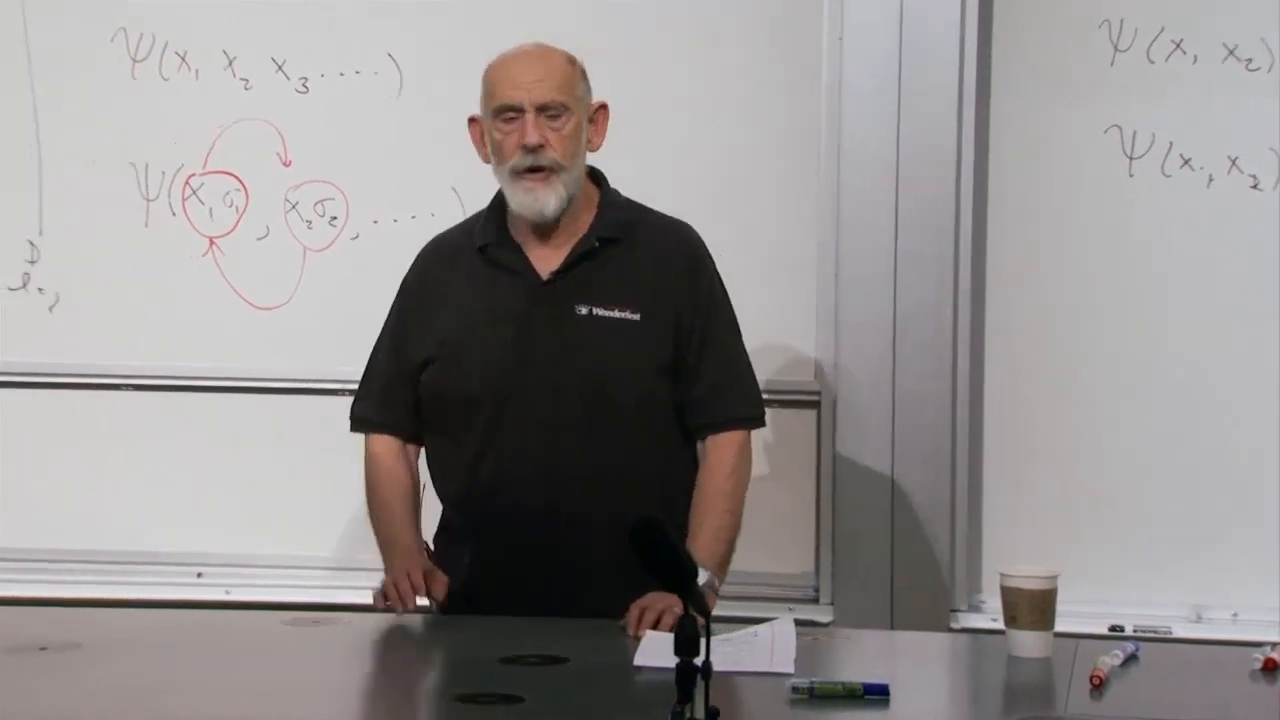
\includegraphics[width=0.9\linewidth]{lecture_05_frame_03.png}
\caption{يبدل تبادل جسيمين متماثلين وسمي الموضع--اللف المغزلي الكاملين الخاصين بهما. تبقى الحالة البوزونية بلا تغير، بينما تتغير إشارة الحالة الفرميونية.}
\lectureframe{00:35:25}
\end{figure}

هذه استخدامات مختلفة للخطية. لجسيم واحد،
\begin{equation}
\alpha\psi_0(x)+\beta\psi_1(x)
\end{equation}
هو تراكب لبديلين. ولجسيمين،
\begin{equation}
\psi_0(x_1)\psi_1(x_2)
\end{equation}
هو سعة جداء على فضاء ذي إحداثيي جسيمين. ويجمع التماثل أو مضادّة التماثل ذلك الجداء مع نظيره الناتج عن التبديل.

\begin{classroomqa}
\lecturetimestamp{00:36:13}
\audiencequestion{هل يؤدي تبديل الجسيمات إلى أثر تداخل؟}
\lecturerresponse{نعم. يمكن فهم انعدام السعة الفرميونية للحالة نفسها على أنه تداخل هدّام بين المساهمتين الناتجتين عن التبديل.}
\end{classroomqa}

\begin{classroomqa}
\lecturetimestamp{00:37:13}
\audiencequestion{هل اشتق Pauli الاستبعاد باستخدام حجة التماثل نفسها؟}
\lecturerresponse{بدأ Pauli من حقيقة تجريبية، ووجد إطارًا رياضيًا يمكن التعبير عنها فيه. ولم يكن في البداية يشتق الاستبعاد من نظرية أكثر أساسية.}
\end{classroomqa}

توفّر مضادّة التماثل الإطار الرياضي الذي تُصاغ فيه قاعدة الاستبعاد التجريبية.

\begin{classroomqa}
\lecturetimestamp{00:39:01}
\audiencequestion{هل يرتبط تداخل تبديل الجسيمات بالتداخل بين المسارات البديلة؟}
\lecturerresponse{نعم. في أحد التاريخين يمر الجسيمان من دون أن يتقاطعا، بينما في تاريخ آخر يتقاطعان فيصل كل منهما إلى وجهة الآخر. وتتجمع السعات للبوزونات، ويمكن أن تلغي بعضها بعضًا للفرميونات.}
\end{classroomqa}

يوفّر التبديل إشارة السالب الأولى. ويوفّر الدوران الثانية.

\section{إشارة السالب الثانية: الدوران بزاوية \texorpdfstring{\(2\pi\)}{2 pi}}

يبدو أن دورة كاملة لا تفعل شيئًا. فكل اتجاه هندسي عادي يعود إلى نقطة بدايته بعد زاوية \(2\pi\). غير أن ما يجب أن يعود هو الاحتمالات وقيم التوقع. أمّا متجه الحالة نفسه فقد يعود مع طور كلي، كما قد يحدث له تحت التبديل.

\begin{classroomqa}
\lecturetimestamp{00:42:12}
\audiencequestion{أي محور يُستخدم للدوران، وهل المولِّد هو العزم الزاوي المداري أم اللف المغزلي أم كلاهما؟}
\lecturerresponse{يمكن اختيار محور خارجي؛ ويؤخذ فيما يلي أنه محور \(z\). والمولِّد هو العزم الزاوي الكلي، بما في ذلك المساهمتان المدارية والمغزلية. ولا يلزم أن يكون اللف المغزلي نفسه موجّهًا على امتداد المحور المختار.}
\end{classroomqa}

\editorialnote{تستخدم صيغ العزم الزاوي في هذا النقاش \(\hbar=1\)، لذا فإن \(m\) هي القيمة الذاتية اللابعدية لـ \(J_z\).}

لنرمز بـ \(\psi(\theta)\) إلى الحالة التي نحصل عليها عندما تتقدم معلمة الدوران خلال زاوية \(\theta\). ووفق الاصطلاح المستخدم هنا،
\begin{equation}
J_z\psi(\theta)
=
-i\frac{\partial}{\partial\theta}\psi(\theta).
\end{equation}
وبالنسبة إلى حالة ذات \(J_z\) محدد،
\begin{equation}
J_z\psi(\theta)=m\psi(\theta).
\end{equation}
وبجمع المعادلتين نحصل على
\begin{equation}
-i\frac{\partial}{\partial\theta}\psi(\theta)
=
m\psi(\theta),
\end{equation}
وحلها هو
\begin{equation}
\psi(\theta)=e^{im\theta}\psi(0).
\end{equation}

القيم المسموح بها لـ \(m\) هي أعداد صحيحة أو أنصاف أعداد صحيحة. ولذلك
\begin{equation}
\psi(2\pi)
=
\begin{cases}
+\psi(0), & m\in\mathbb Z,\\[4pt]
-\psi(0), & m\in\mathbb Z+\tfrac12.
\end{cases}
\end{equation}
وبعد دورة كاملة أخرى،
\begin{equation}
\psi(4\pi)=\psi(0)
\end{equation}
في كلتا الحالتين. هذه هي إشارة السالب الثانية: فالحالة في متعدِّدة عزم زاوي نصف-صحيح تغيّر إشارتها تحت دوران مقداره \(2\pi\).

لا تغيّر الإشارة \(\lvert\psi\rvert^2\)، ولذلك لا تكون مرئية عندما تضرب الحالة بأكملها. ومع ذلك، فإن دورانًا مقداره \(2\pi\) لا يمثله مؤثر الهوية على حالة ذات لف مغزلي نصف-صحيح. ويصبح الفرق قابلاً للرصد عندما تُجعل الإشارة نسبية إلى سعة متماسكة أخرى.

\section{المساران \texorpdfstring{\(2\pi\) و\(4\pi\)}{2 pi و4 pi}}

يمكن إظهار الفرق بين \(2\pi\) و\(4\pi\) من دون مزيد من الجبر. أمسك كوبًا بيد واحدة وأدره دورة كاملة من غير أن تتركه. يعود الكوب إلى وضعه الأصلي، لكن الذراع تكون قد التوت. واصل حتى دورة ثانية، وعندئذ يمكن إعادة الذراع إلى موضعها الأصلي من دون عكس حركة الكوب.

يتضمن إنشاء ذو صلة وضع كرة داخل صندوق وربطها بالصندوق بخيوط. فإدارة الكرة بمقدار \(2\pi\) تترك تشابكًا. وفي الفضاء الثلاثي الأبعاد الاعتيادي، يمكن فك التشابك المرتبط بدوران مقداره \(4\pi\). والشيء ذو الصلة ليس مجرد الوضع النهائي للكرة، بل المسار المتبع عبر فضاء الدورانات.

\begin{classroomqa}
\lecturetimestamp{00:54:22}
\audiencequestion{إذا أُديرت الكرة مرتين حول المحور نفسه، فهل يمكن حقًا فك الخيوط من تشابكها؟ وهل يتطلب ذلك بُعدًا مكانيًا آخر؟}
\lecturerresponse{يمكن فك مسار \(4\pi\) في الفضاء الثلاثي الأبعاد الاعتيادي. فالزمن يقوم بدور معلمة للحركة؛ وليس اتجاهًا مكانيًا آخر. ولا يمكن فك مسار \(2\pi\) بهذه الطريقة، بينما يمكن فك مسار \(4\pi\).}
\end{classroomqa}

تميّز هاتان المظاهرتان بين مسار \(2\pi\) غير تافه ومسار \(4\pi\) قابل للفك، من دون تطوير نظرية صورية لزمرة الدوران.

\section{التبديل والدوران في صورة الحزام}

تقف إشارتا السالب الآن جنبًا إلى جنب. فتبديل فرميونين متماثلين يغيّر إشارة دالتهما الموجية المشتركة. كما أن تدوير حالة واحدة ذات لف مغزلي نصف-صحيح بمقدار \(2\pi\) يغيّر إشارتها أيضًا. ويعطي الحزام علاقة هندسية بين العمليتين.

رتّب الحزام بحيث يكون طرفاه السفليان قد تبدّلا. ومن منظور آخر، يحمل الحزام نفسه لفة بمقدار \(2\pi\). إن إجراء التبديل مع دوران مقداره \(2\pi\) يزيل اللفة ويترك الحزام غير ملتف. ويمكن اختزال العملية المركبة اختزالًا متصلًا إلى ألا نفعل شيئًا.\footnote{تُنسب ملاحظة التبديل--الدوران في المحاضرة إلى David Finkelstein. ولا يحدَّد أي منشور بعينه في سجل المصدر، لذلك أُبقي الاسم هنا على هذا الأساس وحده.}

\begin{classroomqa}
\lecturetimestamp{01:01:12}
\audiencequestion{أهذا مجرد وصف لكيفية تضمين الحزام في الفضاء، لا وصف لطوبولوجيا الجسيمات؟}
\lecturerresponse{يمكن قراءة الحزام بوصفه تاريخًا جسيميًا في الزمكان. ومع سير الزمن إلى الأعلى، يعطي مقطع عرضي خلاله أشياء شبيهة بالجسيمات. تُنشأ أزواج، ويُدار أحد الأجسام بمقدار \(2\pi\)، ويُبدَّل جسمان متماثلان. وفي ذلك التاريخ يلغي طورا الدوران والتبديل أحدهما الآخر.}
\end{classroomqa}

يجعل هذا التاريخ تتبّع الأطوار صريحًا. ابدأ من دون جسيمات. وفي موضعين منفصلين، أنشئ زوجًا جسيم--ضديد جسيم، فيبقى أربعة جسيمات عند زمن وسيط. أدر أحد الجسيمات بمقدار \(2\pi\) بينما تبدّل جسيمين متماثلين في موضع آخر من الترتيب. ويمكن تشويه التاريخ الكامل تشويهًا متصلًا إلى التاريخ الابتدائي الذي فيه يُنشأ زوج ثم يُفنى لاحقًا. وفي تتبّع الإشارات الجاري نقاشه، لا يحمل ذلك التاريخ التافه أي طور إضافي. وإذا كانت \(\eta_{\mathrm{rot}}\) و\(\eta_{\mathrm{ex}}\) ترمزان إلى الإشارتين، أمكن كتابة الإلغاء المذكور بإيجاز على الصورة الآتية\footnote{تسجّل معادلة الطور هذه الإلغاء الموصوف من 01:06:50 إلى 01:07:18؛ وتعرض المحاضرة هذا البناء على أنه موحٍ لا برهان صارم.}
\begin{equation}
\eta_{\mathrm{rot}}\eta_{\mathrm{ex}}=1.
\end{equation}

\begin{classroomqa}
\lecturetimestamp{01:03:34}
\audiencequestion{هل يمكن ربط التبديل بالدورانات بأن نَدَع كلًا من جسيمين يتحرك خلال \(\pi\) ثم نعيد توجيههما؟}
\lecturerresponse{قد يعكس هذا البناء رياضيات ذات صلة، لكنه يستخدم دورانين منفصلين مقدارهما \(\pi\). أمّا العملية التي تُحلَّل هنا فتتضمن دورانًا واحدًا مقداره \(2\pi\)، لذا فالحجتان ليستا متطابقتين.}
\end{classroomqa}

تعتمد الحجة على إمكان إنشاء أشياء شبيهة بالجسيمات وإفنائها. ولن تكون لها هذه الصيغة في نظرية تكون جسيماتها أزلية. وهي أيضًا لا تُقدَّم بوصفها البرهان المعياري على مبرهنة اللف المغزلي--الإحصاء. وغرضها إظهار سبب طوبولوجي لتلاؤم إشارتي التبديل والدوران.

\section{التكتلات، والصور المرآتية، والفناء}

يمكن تكرار هذا البناء مع تشكيلات حقلية موضعية. افترض أن حقلًا واحدًا أو أكثر يأخذ قيم الفراغ الخاصة به في كل مكان تقريبًا، ولكن له شكلًا وبنية غير صفريين في منطقة صغيرة. ذلك التشكيل الموضعي هو تكتل.

الآن أنشئ تشكيلًا ثانيًا بوصفه الصورة المرآتية المناسبة للأول. سمِّ أحدهما الجسيم والآخر ضديد الجسيم. قرّبهما أحدهما من الآخر. تلتقي الأجزاء المتناظرة من التشكيلين الحقليين ويبطل بعضها بعضًا. وفي مرحلة وسطى قد تكون بعض أجزاء التكتلين قد اختفت بالفعل بينما تبقى أجزاء أخرى. ومواصلة التشويه تزيل البنية المتبقية وتعيد الحقول إلى تشكيل الفراغ. وتعطي لفتان متعاكستان في حزام الصورة نفسها: ادفع اللفتين معًا فتنفكان.

يمكن إجراء العملية بالعكس. ويمكن للفضاء الخالي أن ينتج تكتلًا وقرينه المرآتي. ويمكن إنشاء زوجين من هذا النوع، وتدوير أحد التكتلات بمقدار \(2\pi\)، وتبديل تكتلين متماثلين، ثم إفناء الزوجين من جديد. وعندئذ ينطبق الإلغاء نفسه للتبديل--الدوران. ويظل هذا توسيعًا استرشاديًا للبناء، لا مبرهنة بشأن كل إثارة موضعية.

\begin{classroomqa}
\lecturetimestamp{01:11:30}
\audiencequestion{هل توجد تحققات فيزيائية لهذه التشكيلات الحقلية الشبيهة بالكتل؟}
\lecturerresponse{نعم. وتشمل الأمثلة الأنوية في الأوصاف من نمط Skyrmion، والأقطاب المغناطيسية الأحادية، وإثاراتٍ حقلية أخرى شبيهة بالجسيمات.}
\end{classroomqa}

إن صورة الكتلة وصورتها المرآتية هي ما يجعل هذا التعميم مفهومًا. والسمة ذات الصلة ليست أن الشيء بدأ بوصفه جسيمًا نقطيًا أوليًا، بل إن إثارةً شبيهةً بالجسيم وقرينتها يمكن إنشاؤهما، ثم جمعهما معًا، ثم إفناؤهما على نحو مستمر. وهذه السمة تحفز علاقة أوسع بين سلوك الدوران وسلوك التبادل.

\begin{classroomqa}
\lecturetimestamp{01:16:12}
\audiencequestion{هل يعني اللف المغزلي بمقدار نصف أن الحالة تكتسب فقط نصف طور الدوران المعتاد؟}
\lecturerresponse{الطور في هذا الاصطلاح هو \(e^{im\theta}\). وعندما تكون \(m\) نصفَ عددٍ صحيح، فإن دورانًا بمقدار \(2\pi\) يعطي \(-1\)، بينما يعطي دوران بمقدار \(4\pi\) \(+1\).}
\end{classroomqa}

\section{إشارة كلية وتجربة عدمية}

هل يمكن رصد إشارة السالب الناتجة عن دوران بمقدار \(2\pi\)؟ ابدأ بتجربة لا يمكن فيها ذلك. احبس إلكترونًا في مجال مغناطيسي، ودع لفَّه المغزلي يتبع المجال بينما يُدار الجهاز ببطء خلال \(2\pi\)، ثم أطلق الإلكترون إلى جهاز تداخل. وقارن هذا بالإجراء نفسه من دون الدوران.

يغيّر الدوران الحالة على النحو الآتي:
\begin{equation}
\psi\longmapsto-\psi,
\end{equation}
لكن إشارة السالب تضرب الحالة بأكملها. وكل احتمال يبقى بلا تغير، لذلك لا يحتفظ نمط التداخل النهائي بأي أثر لحدوث الدوران التمهيدي أو عدم حدوثه. وهذه تجربة عدمية: فالطور المشترك لا يملك ما يتداخل معه.

\begin{classroomqa}
\lecturetimestamp{01:20:01}
\audiencequestion{لماذا يجب إجراء دوران المجال المغناطيسي ببطء؟}
\lecturerresponse{يجب أن يظل اللف المغزلي متتبعًا المجال المغناطيسي الدائر. فإذا جرى سحب المجال بسرعة أكبر من اللازم، فلن يبقى اللف المغزلي مقترنًا به.}
\end{classroomqa}

\section{إلكترون واحد في فرعين متماسكين}

تصبح الإشارة قابلة للرصد حين تُجعل نسبية. أرسل إلكترونًا واحدًا عبر مقسِّم حزمة. يسلك جزء من دالته الموجية مسارًا، ويسلك جزء آخر مسارًا آخر:
\begin{equation}
\psi(x)=\psi_1(x)+\psi_2(x).
\end{equation}
هذا إلكترون واحد، لا إلكترونان. إنه تراكب متماسك لبديلين. ويجب إبقاء التمييز واضحًا: فالحزمتان ليستا جسيمين مستقلين.

وجّه الحزمتين إلى منطقتين منفصلتين تحتويان على حقول مغناطيسية. أدر المجال في إحدى المنطقتين بمقدار \(2\pi\)، واترك المجال في الأخرى دون تغيير. بالنسبة إلى حالة ذات لف مغزلي نصف صحيح،
\begin{equation}
\psi_1(x)+\psi_2(x)
\longmapsto
\psi_1(x)-\psi_2(x),
\end{equation}
حيث اختيرت تسمية الفرع الذي خضع للدوران على أنها \(2\). والإشارة الآن نسبية. وعندما تتراكب الحزمتان لاحقًا، يكون الجمع قد تحول إلى طرح. ويمكن لنقطة من التداخل البنّاء أن تصبح نقطة من التداخل الهدّام، أو حتى عقدة.

\begin{classroomqa}
\lecturetimestamp{01:23:46}
\audiencequestion{ما الذي يجري تدويره إذا كان هناك إلكترون واحد فقط ولكن فرعان للدالة الموجية؟}
\lecturerresponse{الإلكترون في تراكب متماسك لبديلين موضعيين. أحد الفرعين يُدار والآخر لا يُدار. وإذا فُتحت الصناديق لمعرفة أي البديلين قد وقع، فإن ذلك القياس يدمّر التداخل.}
\end{classroomqa}

إن فتح الصناديق لن يكشف إلا عن إلكترون واحد، في أحد الصندوقين أو الآخر. ومن دون ذلك القياس تبقى كلتا السعتين في الحالة. ويؤدي تكرار التجربة إلى تراكم نمط التداخل كشفًا بعد كشف. وعند عقدة تنتج عن إشارة السالب النسبية، لا يُكشف عن أي إلكترون.

\section{السبق المغناطيسي وتداخل الشقين}

يستعاض عن تجربة الصندوق البطيئة جدًا بترتيب تخطيطي أكثر عملية. قسّم موجة إلكترون متماسكة إلى مسارين. وفي أحد المسارين، دع الإلكترون يمر عبر منطقة مغناطيسية يكون لفّه المغزلي فيها، في البداية، متعامدًا على المجال. عندئذ يسبق اللف المغزلي. وباختيار شدة المجال وزمن العبور، يمكن للّف المغزلي في ذلك الفرع أن ينجز لفة كاملة بمقدار \(2\pi\)، بينما لا يخضع الفرع الآخر لمثل هذه اللفة.\footnote{تنص المحاضرة على أن تجربةً ذات صلة بطور السبينور قد أُجريت، وتصف مبدأها، لكن السجل المصدري لا يحدّد ورقةً بحثية ولا جهازًا بعينه. ولذلك يقتصر العرض هنا على البنية المعطاة في المحاضرة.}

\begin{classroomqa}
\lecturetimestamp{01:27:05}
\audiencequestion{كيف يمكن تحديد مسار الإلكترون المنفرد؟}
\lecturerresponse{لا يمكن تحديده من دون إفساد التجربة. فأي قياس يسجّل أيَّ مسار سلكه الإلكترون يدمّر التداخل.}
\end{classroomqa}

\begin{classroomqa}
\lecturetimestamp{01:27:50}
\audiencequestion{ما المقصود بدقة بفرع من الدالة الموجية، وكيف يُنتج المقسِّم فرعين؟}
\lecturerresponse{الفرع حزمة موجية متموضعة على امتداد أحد المسارين. ويحوّل المقسِّم الموجة الداخلة إلى حزمتين منفصلتين مكانيًا، ويمكن لحقول كهربائية أو مغناطيسية أن توجه هاتين الحزمتين على مسارات مختلفة.}
\end{classroomqa}

باستثناء المنطقة المغناطيسية، هذه هي تجربة الشقين. تنفصل موجة إلكترون داخلة إلى حزمتين. وتنتشر الموجتان الخارجتان إلى منطقة كشف مشتركة، حيث تتراكب سعتاهما. ومن دون دوران نسبي قد تتضافر السعات المركزية. أما دوران اللف المغزلي بمقدار \(2\pi\) في أحد المسارين فيعكس إشارة إحدى السعات، ويمكن أن يجعل المساهمات نفسها تلغي بعضها بعضًا.

\begin{classroomqa}
\lecturetimestamp{01:30:46}
\audiencequestion{كيف يمكن أن يحدث تداخل إذا كان الإلكترون ينتقل عبر أنابيب أو شقوق منفصلة؟}
\lecturerresponse{إن الكشف النهائي لا يكشف عن المسار. تنتشر سعتا الموجة الخارجتان وتتراكبان عند الكاشف. أما النظر لمعرفة أيَّ مسار قد سلكه فسيُفسد التداخل.}
\end{classroomqa}

\begin{classroomqa}
\lecturetimestamp{01:33:22}
\audiencequestion{هل يجب أن يكون قطر الأنبوب أو الشق مقارنًا بطول موجة الإلكترون؟}
\lecturerresponse{في تحقيق حرفي لتجربة الشقين قائم على الحيود، يجب أن تكون الفتحة صغيرة بما يكفي لإنتاج الانتشار المطلوب. أما الجهاز الموصوف هنا فهو تخطيطي لا تصميم عملي.}
\end{classroomqa}

\begin{classroomqa}
\lecturetimestamp{01:33:44}
\audiencequestion{هل يترك دوران استقطاب الفوتونات الموافق بمقدار \(2\pi\) نمط التداخل من دون تغير؟}
\lecturerresponse{نعم. فالفوتونات ذات لف مغزلي صحيح، ولذلك فإن دورانًا كاملاً بمقدار \(2\pi\) لا يُدخل إشارة السالب الفرميونية.}
\end{classroomqa}

\begin{classroomqa}
\lecturetimestamp{01:34:12}
\audiencequestion{ما الاختلاف الطفيف بين التجربة العملية والنسخة المثالية؟}
\lecturerresponse{في البناء المثالي يُدار اللف المغزلي أديباتيًا. أما في الوصف العملي فيتحرك الإلكترون عبر منطقة مغناطيسية ويسبق لفّه المغزلي بسرعة أكبر، لكن الطور المقاس يظل هو الطور المرتبط بلفة مقدارها \(2\pi\).}
\end{classroomqa}

يعزل الترتيب البطيء الفكرةَ بضمان أن اللف المغزلي يتبع المجال من دون حركة إضافية. ويصل ترتيب السبق إلى الإشارة النسبية نفسها ديناميكيًا. وفي أيٍّ من النسختين، يجب أن يكفّ المساران عن كونهما قابلين للتمييز قبل أن يظهر نمط تداخل.

\begin{classroomqa}
\lecturetimestamp{01:36:15}
\audiencequestion{هل يجب إعادة جمع الفرعين بعد المقسِّم؟}
\lecturerresponse{نعم. يجب أن تتراكب الحزمتان الموجيتان الناشئتان، أو أن تنتشرا على منطقة كشف مشتركة، بحيث تستطيع سعتاهما تكوين نمط تداخل.}
\end{classroomqa}

\begin{classroomqa}
\lecturetimestamp{01:38:12}
\audiencequestion{هل تجربة دوران الإلكترون الواحد هذه نتيجة لمبدأ استبعاد باولي؟}
\lecturerresponse{لا. فهناك إلكترون واحد فقط. تقيس التجربة طور السبينور تحت الدوران، لا استبعاد فرميونين من حالة واحدة.}
\end{classroomqa}

\section{تداخل التبادل والدوران النسبي}

يمكن كشف إشارة التبادل بالطريقة العامة نفسها، مع أن الجهاز المقترح أعقد. ابدأ بإلكترونين وقسّم دالتهما الموجية المشتركة إلى فرعين متماسكين. وما يزال هناك إلكترونان فقط، لا أربعة: فالزوج يسلك أحد البديلين أو الآخر. أجرِ تبادلاً بين الإلكترونين في أحد الفرعين واتركهما في الآخر من دون تبادل. وبعد إعادة جمع الفرعين، تظهر إشارة التبادل الفرميونية بوصفها طورًا نسبيًا، ويمكنها أن تغيّر التداخل.

يقارن الاقتراح الأخير بين إشارتي السالب مباشرةً. يكتسب أحد الفرعين طور التبادل الفرميوني، بينما يكتسب الآخر طور الدوران الموافق بمقدار \(2\pi\). وكلا الطورين يساويان \(-1\)، ولذلك يزول الأثر النسبي.\footnote{يوضح التسجيل بين 01:40:26 و01:41:15 بوضوح طورَ تبادل، وطورَ دوران بمقدار \(2\pi\)، وإلغاءَ أحدهما للآخر، لكن التعيين التفصيلي للدوران لا يمكن استخلاصه من الكلام المتاح.} وتعرض المحاضرة هذا على أنه تجربة فكرية مقترحة، وتقول إنه، بحسب علم المتحدث، لم تُجرَ.

\begin{classroomqa}
\lecturetimestamp{01:41:34}
\audiencequestion{هل إن رصد طور تبادل من شأنه أن يُشكِّك في عدم قابلية التمييز بين الإلكترونين؟}
\lecturerresponse{لا. إن عدم قابلية التمييز الكمومي أدق من التطابق الكلاسيكي. فهو يسمح لمتجه الحالة بأن يغيّر إشارته تحت التبادل، مع أنه لا يوجد أي وسم قابل للرصد يميّز بين الجسيمين.}
\end{classroomqa}

هناك قيد أخير. إن تدوير عالمٍ معزولٍ بأكمله بمقدار \(2\pi\) لن يسفر إلا عن طورٍ مشترك، ولن تستطيع أي تجربة داخلية كشفه. أما التجربة القابلة للرصد فتُخضِع أحد الفرعين المتماسكين لدوران بالنسبة إلى الآخر. ولذلك فإن ما يُرصَد ليس إشارةً مطلقة، بل التداخل الناجم عن إشارة نسبية.
